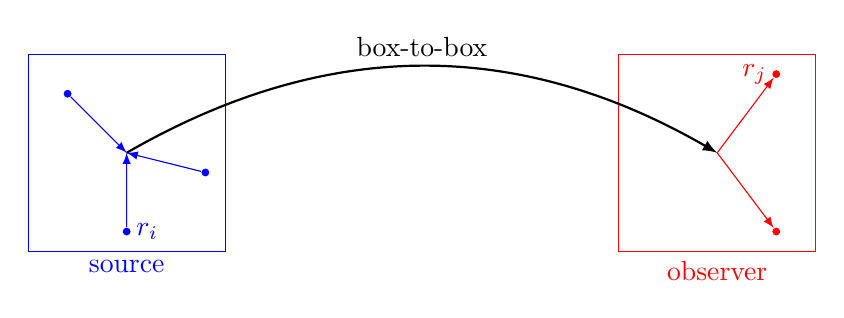
\begin{tikzpicture}[scale=2.5, >=latex]
  \draw[color=blue] (0, 0) rectangle (1, 1);
  \draw[color=red] (3, 0) rectangle (4, 1);

  \draw[color=blue] (0.2, 0.8) node[circle, fill, inner sep=1pt](s1){};
  \draw[color=blue] (0.5, 0.1) node[circle, fill, inner sep=1pt](s2){};
  \node[blue, anchor=west] at (s2) {$\vb{r}_i$};
  \draw[color=blue] (0.9, 0.4) node[circle, fill, inner sep=1pt](s3){};

  \draw[color=red] (3.8, 0.9) node[circle, fill, inner sep=1pt](o1){};
  \node[red, anchor=east] at (o1) {$\vb{r}_j$};
  \draw[color=red] (3.8, 0.1) node[circle, fill, inner sep=1pt](o2){};

  \draw[color=blue, ->] (s1) -- (0.5, 0.5);
  \draw[color=blue, ->] (s2) -- (0.5, 0.5);
  \draw[color=blue, ->] (s3) -- (0.5, 0.5);

  \draw[color=red, ->] (3.5, 0.5) -- (o1);
  \draw[color=red, ->] (3.5, 0.5) -- (o2);

  \draw[->, thick] (0.5, 0.5) to [bend left] node[pos=0.5, above]{box-to-box} (3.5, 0.5);

  \node[blue, anchor=north] at (0.5, 0) {source};
  \node[red, anchor=north] at (3.5, 0) {observer};
\end{tikzpicture}
